\documentclass{article}
\usepackage{graphicx}
\usepackage{hyperref}
\usepackage{amsmath}

\begin{document}

\begin{titlepage}
    \begin{center}
        \vspace*{1cm}
            
        \Huge
        \textbf{Electricity Usage Optimizer}
            
        \vspace{0.5cm}
        \LARGE
        Miniproject Report
        
        \date{today}
            
        \vspace{1.5cm}
            
        Pontus Hedlund, Sanna Korpi, Topi Ranta
            
        \vfill
            

            
        \vspace{0.8cm}
            
            
        \Large
        University of Helsinki\\
        Introduction to Data Science\\
        31.10.2022\\
            
    \end{center}
\end{titlepage}

\tableofcontents

\section{A Simple Prediction of Electricity Price Development}
\label{section:introduction}

%% summary of idea w/ references to repository, application, presentation
%% summary of the data and the technical solution

The rest of the report is composed as follows: the data used and data preprocessing is described in Chapter \ref{section:data}. The prediction formulation and the linear regression model used in the project are presented in Chapter \ref{section:analysis}. User experience and results delivery for the end user 

\section{Data}
\label{section:data}

\subsection{Data Used in the Project}
\label{subsection:datadescription}

\begin{enumerate}
    \item Fingrid: Wind Power Production Data
    
    https://data.fingrid.fi/en
    
    \item Helen District Heating Power Data
    
    https://www.helen.fi/en/company/responsibility/current-topics/open-data
    
    \item Entsoe Day-ahead Market price history and current prices
    
    https://transparency.entsoe.eu
    
    \item Finnish Meteorological Institute Weather Observation Data for Kumpula, Helsinki.
    
    https://en.ilmatieteenlaitos.fi/open-data
    
\end{enumerate}

The data for all sources mentioned above is available publicly in CSV format. We chose to downlaod data spanning from the beginning of 2019 as far ahead as possible. For Helen, the data ends at the end of year 2021. For predictions, we are fetching the most recent data in addition.

\subsection{Exploratory Data Analysis and Data Preprocessing}
\label{subsection:eda}

We created Jupyter Notebooks for all data sources to clean and process the data. The products of this process was datasets with the datetime field as index. Two separate tables were created for each data source - historical and a time series forecast. The historical data is used for training the model, and the forecast combined with available amendments from APIs to construct the final predicted price.

\subsection{Data Warehousing and Data Protection}
\label{subsection:wareousing}

All data used for our purpose is publicly available. No data subject to the GDPR act is used, since we are not collecting any data for individuals.

\section{Data Analysis}
\label{section:analysis}

%% target value
\subsection{Feature Extraction}
\label{subsection:extraction}

Features extracted for the model were:

'WindMWh', 'ConsumptionMWh', 'pressure', 'rain', 'humidity',

'temperature', 'wind' and the target value was 'price'.


\subsection{Gathering the Data for the Prediction}
\label{subsection:datafilling}

Since the model is trained on past data, all the same variables need to be present when performing the prediction. Since all of these are not available for the prediction time, we created time series forecasts that should give a best estimate of the values (See figure \ref{fig:consumption}).

\begin{figure}
    \centering
    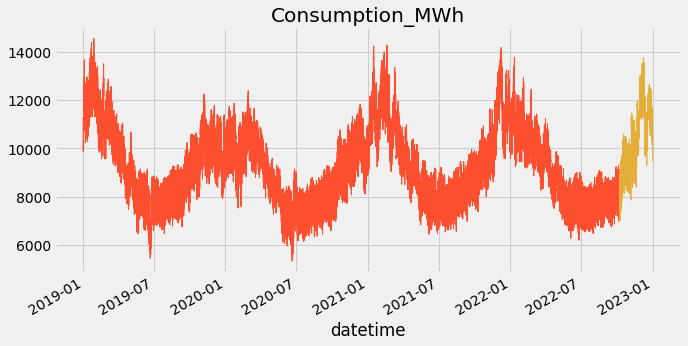
\includegraphics[width=15cm]{report/images/consumption.png}
    \caption{Time series for Consumption in MWh with historical data in red and the forecast in orange.}
    \label{fig:consumption}
\end{figure}

\subsection{Time Series Prediction with XGBoost}
\label{subsection:xgboost}

The ML model used for this application is the XGBoost Regressor, which is an ensemble method based on gradient-boosted decision trees. It was found to be very fast to train and very accurate.

When training the forecasts, we used cross validation with time series splits (See figure \ref{fig:ts-cross-validation}).

\begin{figure}
    \centering
    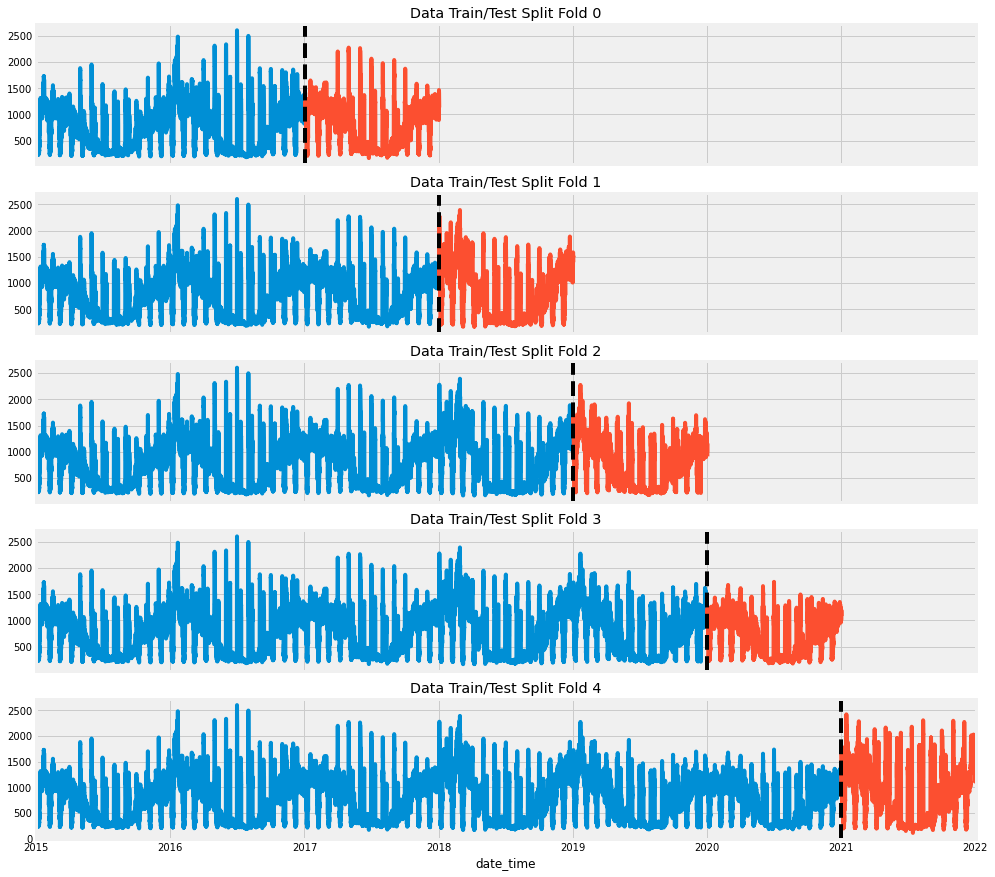
\includegraphics[width=15cm]{report/images/ts-cross-validation.png}
    \caption{Cross validation using Time Series Splits with each split being a year.}
    \label{fig:ts-cross-validation}
\end{figure}



\section{Delivering Results for the End User}
\label{section:delivery}

We calculate a simple moving average (SMA) of the electricity price with a window of 168 hours (7 days) to create a reference price point. For each prediction time, we compare the predicted or known price to the index via equation \ref{eq:index}.


\begin{equation} \label{eq:index}
\text{"Price Index"}_i = \frac{\text{SMA}_i}{\text{"Predicted Price"}_i}
\end{equation}

The price index is then classified as follows:

\begin{enumerate}
    \item $\text{"Price Index"}_i < 0.8$ : "Boost"
    \item $0.8 \leq \text{"Price Index"}_i \leq 1.2$ : "Maintain"
    \item $\text{"Price Index"}_i > 1.2$ : "Restrict"
\end{enumerate}

\subsection{Web Application}
\label{subsection:server}

Our deliverable is a web application built with FastAPI that serves a landing page and a page for planning. The plan page shows a table with hourly times for the next 36 hours with a recommendation and the price index. The whole package is available on Github at https://github.com/IDS-mini/electricity .

\subsection{Visualization and User Experience}
\label{subsection:ux}

%% no gdpr data gathered from the user either

\section{Conclusions}
\label{section:conclusions}

%% what was achieved
%% what was learned
%% what we would do differently
%% ideas for further development or research


\end{document}

